\documentclass[10pt]{beamer}
\usepackage{pgfpages}

%% FOR DRAFT: %%%%%%%%%%%%%%%%%%%%%%%%%%%%%%%%%%%%%%%%%%%%%%%%%%%%%%%%
%% Comment the first line and uncomment the next lines:
%\documentclass[draft,10pt]{beamer}
%%%%%%%%%%%%%%%%%%%%%%%%%%%%%%%%%%%%%%%%%%%%%%%%%%%%%%%%%%%%%%%%%%%%%%

%% FOR HANDOUT: %%%%%%%%%%%%%%%%%%%%%%%%%%%%%%%%%%%%%%%%%%%%%%%%%%%%%
%% Comment the first line and uncomment the next lines:
% \documentclass[handout,10pt]{beamer}
% \usepackage{pgfpages}
% \pgfpagesuselayout{2 on 1}[a4paper,border shrink=5mm]
%% The previous line set 2 slide on 1 paper, if you change the number,
%% you can change the slide for sheet.
%%%%%%%%%%%%%%%%%%%%%%%%%%%%%%%%%%%%%%%%%%%%%%%%%%%%%%%%%%%%%%%%%%%%%%


% This file is a solution template for:

% - Talk at a conference/colloquium.
% - Talk length is about 20min.
% - Style is ornate.

\mode<presentation>
{
  \usetheme{Hannover}
%  \usecolortheme{rose}
  \usecolortheme{default}
  \setbeamercovered{transparent}
}
\usepackage[absolute,overlay]{textpos}

\usepackage{etex}
%\usepackage[italian]{babel}
\usepackage[utf8]{inputenc}
\usepackage{times}
\usepackage[T1]{fontenc}
\usepackage{hanging}

\usepackage{multimedia}
%\usepackage{movie15}
%\usepackage{flashmovie}

%%%%%%% Other Packages %%%%%%%

% To include image
%\usepackage{graphics} %Gia introdotto da beamer
%----------------------

% To draw
\usepackage{tikz}
%--- tikz libraries
\usetikzlibrary{arrows}
\usetikzlibrary{decorations.pathmorphing}
\usetikzlibrary{shapes}
\usetikzlibrary{mindmap}
\usetikzlibrary{er}
\usetikzlibrary{shadows}
%--- tikz colordef
\definecolor{bluepres}{RGB}{215,215,240}
\definecolor{bluebold}{RGB}{51,51,179}
\definecolor{red}{RGB}{245,10,39}
%----------------------

% Nice Boxex
\usepackage{fancybox}
%----------------------

% Chemical Pacages
%\usepackage{m-ch-en}
%\usepackage{m-pictex}
%----------------------

% For Comment Environment
\usepackage{verbatim}
%\usepackage{gnuplottex}

%----------------------

% To improve my tables
\usepackage{booktabs}
\usepackage{tabularx}
\usepackage{multirow}
%\usepackage{colortbl}
%----------------------

% To improve my itemize
%\usepackage{enumitem}
%\setlist{nolistsep,leftmargin=*}
%----------------------

% For a better style
%\usepackage{microtype}
%----------------------

% To edit the linespread
%\usepackage{setspace}
%----------------------

%\begin{comment}
%For measure unit (SI)
%\usepackage [squaren,italian,textstyle,thinqspace,thickspace]{SIunits}
%----------------------

%For Math tools
\usepackage{amsmath}
\usepackage{mathtools}
\usepackage{mathrsfs}

%----------------------


\usepackage{xparse}
\ExplSyntaxOn
\DeclareExpandableDocumentCommand{\convertlen}{ O{cm} m }
 {
  \dim_to_decimal_in_unit:nn { #2 } { 1 #1 } cm
 }
\ExplSyntaxOff

\usepackage[style=chem-acs]{biblatex}
%\usepackage[style=authoryear-comp, backend=biber]{biblatex}
\addbibresource{library.bib}
\renewcommand*{\footnotesize}{\scriptsize}
\renewcommand{\thefootnote}{\fnsymbol{footnote}}


%%%%%%%%%%%%%%%%%%%%%%%%%%% My Own Command %%%%%%%%%%%%%%%%%%%%%%%%%%%

%
% abbreviations for text
%------------------------------
\newcommand{\eng  }[1]{\emph{#1}}
\newcommand{\soft }[1]{\emph{#1}}
%\newcommand{\sep }[1]{\; #1 \;}
%\newcommand{\soft}[1]{\MakeUppercase{#1}}

%
% abbreviations for mathmatics
%------------------------------
\newcommand{\pd       }[2]{\frac{\partial #1}{\partial #2}}
\newcommand{\mtx      }[1]{\underline{#1}}
\newcommand{\diver    }[1]{\vnabla \scaltimes #1}
\newcommand{\vnabla   }   {\vec{\nabla}}
\newcommand{\scaltimes}   {\cdot}
\newcommand{\lapl     }[1]{\vnabla^2 #1}
\newcommand{\trasp    }[1]{{#1}^T}
\newcommand{\is       }[1]{{#1}'}
\newcommand{\phs      }[1]{\overline{#1}}
\newcommand{\e        }   {\mathrm{e}}                       % Nepero's numeber
\newcommand{\intd     }   {\,\mathrm{d}}                     % Integration variable


%
% abbreviations for enviroments
%------------------------------
\newcommand{\bec}{\begin{center}}
\newcommand{\enc}{\end{center}}
\newcommand{\ber}{\begin{flushright}}
\newcommand{\enr}{\end{flushright}}
\newcommand{\beq}{\begin{equation}}
\newcommand{\eeq}{\end{equation}}
\newcommand{\bit}{\begin{itemize}}
\newcommand{\eit}{\end{itemize}}

%
% abbreviations for chemistry
%------------------------------
\newcommand{\ch}[1]{\chemical{#1}}

%
% abbreviations for tikz shape
%------------------------------
\newcommand{\hence}[3]{  % freccia larga si specifica la larghezza,
                         % lunghezza e i gradi di rotazione.
  \bec
  \tikz{\node[single arrow,draw=bluebold,thick,rotate=#3,minimum
    width=#1,minimum height=#2,fill=bluepres!94]{};}
  \enc
}

\newcommand{\textarrow}{
  \tikz[baseline]{
    \draw[->,shorten >=1pt,>=stealth,thick]
    (0,.5ex) -- ++(8mm,0);}
}

\newcommand{\uptextarrow}[1]{
  \tikz[baseline=0.1ex]{
    \draw[->,shorten >=1pt,>=stealth,thick,rotate=90]
    (0,0ex) -- ++(#1,0);}
}

\newcommand{\downtextarrow}[1]{
  \tikz[baseline=-1.5ex]{
    \draw[->,shorten >=1pt,>=stealth,thick,rotate=-90]
    (0,0ex) -- ++(#1,0);}
}


%
% my environments
%------------------------------

\newcommand{\myitem}[1]
{
  \begin{footnotesize}
    \begin{tikzpicture}[baseline,inner sep=0]
      \node[circle,minimum width=1ex,draw=bluebold,shading=ball,/tikz/ball color=bluebold] at (0,0){};
      \draw (0ex,0ex)
      node[right,text width=0.9\textwidth,rounded corners,draw=bluebold,fill=bluepres!94,inner sep=1ex]
      {#1};
    \end{tikzpicture}
  \end{footnotesize}
}

\newcommand{\myalertitem}[1]
{
  \begin{footnotesize}
    \begin{tikzpicture}[baseline,inner sep=0]
      \node[circle,minimum width=1ex,draw=red,shading=ball,/tikz/ball color=red] at (0,0){};
      \draw (0ex,0ex)
      node[right,text width=0.9\textwidth,rounded corners,draw=red,fill=red!40,inner sep=1ex]
      {#1};
    \end{tikzpicture}
  \end{footnotesize}
}

\newcommand{\myblock}[1]
{
  \begin{footnotesize}
    \begin{tikzpicture}[baseline,inner sep=0]
%      \node[circle,minimum width=1ex,draw=bluebold,fill=bluebold] at (0,0){};
      \draw (0ex,0ex)
      node[right,text width=0.9\textwidth,rounded
      corners,draw=bluebold,fill=bluepres!94,inner sep=1ex,text centered]
      {#1};
    \end{tikzpicture}
  \end{footnotesize}
}

\newcommand{\mywhiteblock}[1]
{
  \begin{footnotesize}
    \begin{tikzpicture}[baseline,inner sep=0]
%      \node[circle,minimum width=1ex,draw=bluebold,fill=bluebold] at (0,0){};
      \draw (0ex,0ex)
      node[right,text width=0.9\textwidth,rounded
      corners,draw=bluebold,fill=white,inner sep=1ex,text centered]
      {#1};
    \end{tikzpicture}
  \end{footnotesize}
}

\newcommand{\myalertblock}[1]
{
  \begin{footnotesize}
    \begin{tikzpicture}[baseline,inner sep=0]
      \node[circle,minimum width=1ex,draw=red,shading=ball,/tikz/ball color=red] at (0,0){};
      \node[circle,minimum width=1ex,draw=red,shading=ball,/tikz/ball color=red] at (9.5,0){};
      \draw (0ex,0ex)
      node[right,text width=0.9\textwidth,rounded
      corners,draw=red,fill=red!15,inner sep=1ex, text centered]
      {#1};
    \end{tikzpicture}
  \end{footnotesize}
}

%%%%%%%%%%%%%%%%%%%%%%%%%%%%%%%%%%%%%%%%%%%%%%%%%%%%%%%%%%%%%%%%%%%%%%
\graphicspath{{../img/}}

\title[] % (optional, use only
                                % with long paper titles)
{Short i-PI tutorial}

%\logo{\inlcudegraphics[width=10cm]{LCMD-logo}}
\institute{
%  \vspace{0.4cm}\\
%  
\includegraphics[width=6cm]{EPFL-logo} \\
% \vspace{2ex}
% \textbf{\large{LCMD - EPFL}}\\
% \vspace{1ex}
%  Corso di Laurea Magistrale in Scienze Chimiche
% \vspace{1cm}
  \raisebox{0.03cm}{
\includegraphics[width=0.3\textwidth]{general/group-logo}}
\begin{tabular}{cc}
%  \hline
%  \vspace{-0.1cm}
  \raisebox{0.03cm}{
\includegraphics[width=0.3\textwidth]{general/MAX-logo}} &
  
\includegraphics[width=0.4\textwidth]{general/EPFL-logo-notext}
\end{tabular}\\
\vspace{1em}

ICTP Trieste
}

\date[26.01.2017]
{Riccardo Petraglia\\
26 January 2017}

\subject{Theoretical Computer Science}

%% Per Vedere l'indice all'inizio di ogni sezione
% \AtBeginSubsection[]
% {
%   \begin{frame}<beamer>{Outline}
%     \tableofcontents[currentsection,currentsubsection]
%   \end{frame}
% }

% \AtBeginSection[]
% {
%   \begin{frame}<beamer>{Outline}
%     \tableofcontents[currentsection,currentsubsection]
%   \end{frame}
% }


% If you wish to uncover everything in a step-wise fashion, uncomment
% the following command:
%\beamerdefaultoverlayspecification{<+->}

%\setbeameroption{show notes on second screen=left}
%\setbeameroption{show only notes}
%\setbeamercolor{note page}{bg=white, fg=black}

\newcommand{\unilogo}{
  \setlength{\TPHorizModule}{1pt}
  \setlength{\TPVertModule}{1pt}
   % textblock{}{x,y}: pos(x) = leftUpperCorner + (x *
   % \TPHorizModule), pos(y) = leftUpperCorner - (y * \TPVertModule)
  \begin{textblock}{1}(0.75,230)
   
\includegraphics[width=1.5cm]{general/MAX-logo}
  \end{textblock}
  \begin{textblock}{1}(1,250)
   
\includegraphics[width=1.5cm]{general/EPFL-logo}
  \end{textblock}
  \begin{textblock}{1}(1.5,8)
   
\includegraphics[width=1.5cm]{general/group-logo}
  \end{textblock}
  }

\setbeamertemplate{navigation symbols}{}
\setbeamertemplate{footline}{\unilogo}
%\end{comment}

\begin{document}
%\logo{\includegraphics[width=10cm]{LCMD_logo}}

\begin{frame}
  \titlepage
\end{frame}

\note{
Buonpomeriggio, I'm Riccardo Petraglia. My master thesis is on
simulations of molecules constituent heparin.
}

% \begin{frame}{Outline}
%   \unilogo
%   \tableofcontents[pausesections]
% % You might wish to add the option [pausesections]
% \end{frame}

% \note{
% My talk provides a brief introduction on the importance and on features of
% heparin, after that, I will describe the approach used for simulations
% and then I will show results obtained  and connections between
% simulation results and experimental data. Finally, I will propose some
% possible insights of this work.
% }

\section{Introduction}
\begin{frame}{What is i-PI?}
 \begin{columns}
   \column{0.6\textwidth}
   \begin{itemize}
   \item Universal force engine interface
     \vspace{0.3cm}
   \item Written in Python
     \vspace{0.3cm}
   \item (not-only) with \emph{ab-initio}
     force-evaluators
   \end{itemize}
   \column{0.4\textwidth}
   
\includegraphics[width=\columnwidth]{ipi}
 \end{columns}
\end{frame}

\begin{frame}{How i-PI works}
  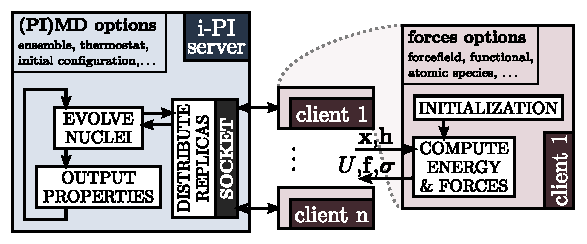
\includegraphics[width=\columnwidth]{ipi-scheme}

  \begin{columns}
    \column{0.5\textwidth}
    \begin{block}{Goal}
      Decouple the problem of evolving the ionic positions and the
      problem of computing the inter-atomic forces.
    \end{block}
    \column{0.5\textwidth}
    \begin{itemize}
      \item i-PI and force calculator on different machine
      \item Crash-safe mechanism
      \item Faster than a ``script'' interface
      \item Easy to parallelize with many replicas
    \end{itemize}
  \end{columns}
\end{frame}

\section{i-PI input}

\begin{frame}{A look at the i-PI input}
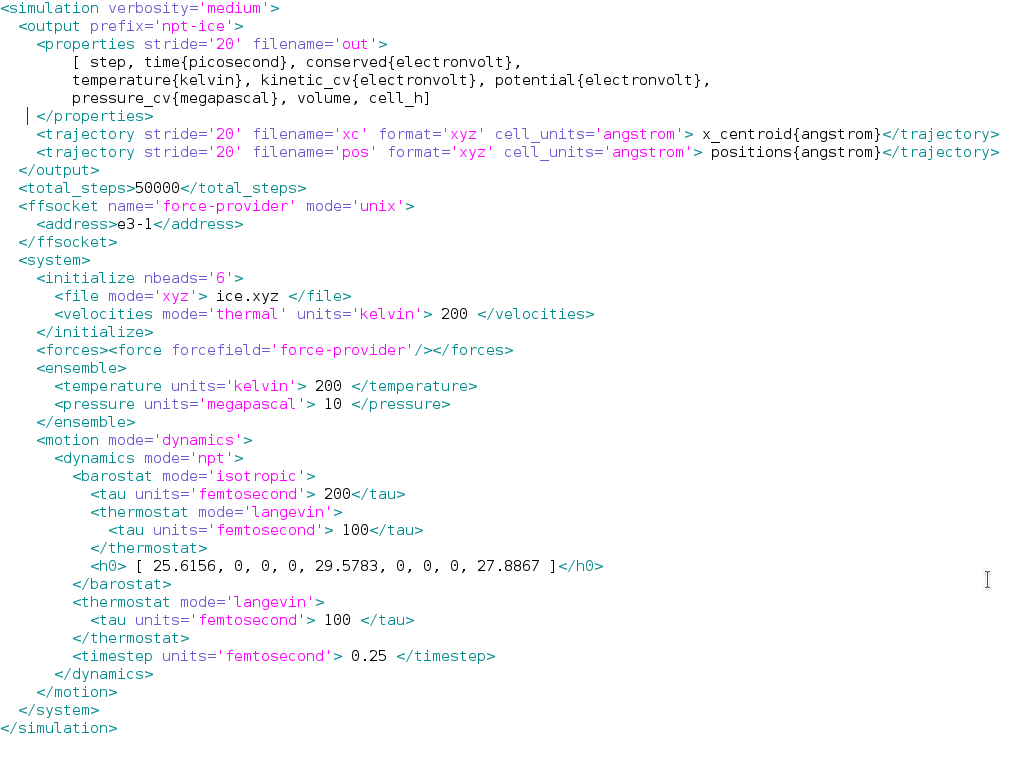
\includegraphics[width=\textwidth]{input_big}
\end{frame}

\begin{frame}{A look at the i-PI input}
\begin{block}{\small XYZ header}
\vspace{1em}
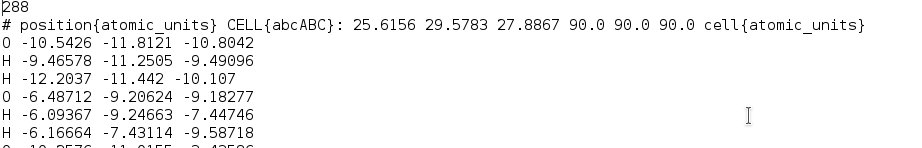
\includegraphics[width=\textwidth]{xyz_header}
\end{block}
\vspace{2.5em}
\begin{block}{\small PDB header}
\vspace{1em}
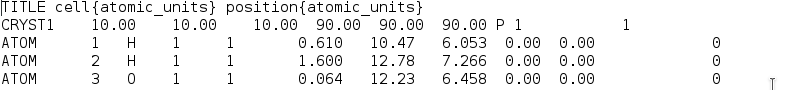
\includegraphics[width=\textwidth]{pdb_header}
\end{block}
\end{frame}

\begin{frame}
Let's start the tutorial\ldots \\
\vspace{2em}
\ldots remember
I am here to answer your questions\ldots
\end{frame}

% \begin{frame}{The Ultimate Goal}
%   \begin{columns}
%     \column{0.5\textwidth}
%     \begin{block}{\small Goals}
%       \small
%       \begin{itemize}
%       \item Reliable and fast approach tuned for organic
%         electronics
%       \item Supramolecular structure description
%       \item Description of challenging systems
%       \end{itemize}
%     \end{block}
%     \vspace{-.4cm}
%     \begin{block}{\small Tools}
%       \small
%       \begin{itemize}
%       \item Dispersion Correction: dDMC\setcounter{footnote}{0}\footnotemark
%       \item REMD@DFTB3\setcounter{footnote}{1}\footnotemark \& REMD@DFTB3-evo\setcounter{footnote}{2}\footnotemark
%       \item New DFA: $\omega$B97X-dDsC\setcounter{footnote}{3}\footnotemark
%       \end{itemize}
%     \end{block}
%     \column{0.5\textwidth}
%     \includegraphics[width=\columnwidth]{intro/nano_solved}
%   \end{columns}
%   \setcounter{footnote}{1}\footnotetext{Petraglia, R.; Steinmann, S.;
%     Corminboeuf, C.\hspace{.5em} \emph{Int. J. Quant. Chem.}
%     \textbf{2015}, \emph{115}, 1265}
%   \setcounter{footnote}{2}\footnotetext{Petraglia, R. \emph{et al.}
%     \hspace{.5em}\emph{J. Comput. Chem.} \textbf{2016}, \emph{37}, 83}
%   \setcounter{footnote}{3}\footnotetext{\textcolor{gray}{Petraglia,
%       R.; Ceriotti, M.; Corminboeuf, C.\hspace{.5em} \emph{In Preparation}}}
%   \setcounter{footnote}{4}\footnotetext{\textcolor{gray}{Fabrizio, A.;
%       Petraglia, R.; Corminboeuf, C.\hspace{.5em} \emph{In Preparation}}}

% \end{frame}

% \note
% {

% \scriptsize Description of the picture.

% We want to develop a QM/MM approach able to describe this kind of
% systems. DFT-MD is computationally too expensive while MM is not able
% to describe the charge mobility: Actually this property make these
% systems so interesting since supramolecular complexes like this can be
% used in organic electronic frameworks.

% We want to go further a merely description of this systems: we want
% understand which are the geometrical key factors (like distance,
% relative orientation, horizontal displacement)
% between $\pi$-delocalized structures, that can improve the charge
% mobility throughout the $pi$-stacked moieties.

% Since DFT cannot be use in large systems, we will use DFTB: that is a
% DFT approximation,  to generate Molecular Dynamics trajectories for
% the big system. Akin to DFT, DFTB suffer for lack of dispersion
% interaction that are really important if we want to study
% $\pi$-stacked systems. The first goal is develop a dispersion correction
% straightforwardly applicable to DFTB scheme. After that we will
% \textcolor{red}{the Verb is missing} the Block-localized wavefunction
% scheme to DFTB in order to be able to use the Marcus-hush theory in
% computing charge mobility.

% To have a finer description of the electronic structure of our system,
% we will provide DFT calculation. Nowadays DFT suffers from two
% challenging shortcoming: charge delocalization error and missing of
% dispersion interactions. To minimize CDE and provide a correction for
% dispersion interaction, we will \textcolor{red}{some verb} a new
% functional based on the existing wB97 and the dDsC dispersion
% correction recently developed at LCMD.

% We assume that reaching this three major achievement will allow the
% description of supramolecular systems organic electronics related and
% the study of those factors able to control the charge mobility in the
% systems.
% }



% \section{test}
% \begin{frame}{dDMC}
% asd\footfullcite{Petraglia2013}
% {\tiny asdasd}
% \end{frame}

\end{document}
